\chapter{PROPOSED METHODOLOGY}
\label{ChapterResearchMethodology}

This chapter presents the complete technical methodology of TemporalAML, covering the dataset, preprocessing pipeline, temporal graph construction, learnable Fourier time encoding, Temporal Graph Attention Network architecture, multi-pattern AML detection heads, and per-pattern subgraph explainability. The chapter is structured to follow the four research objectives.

---

\section{Problem Formulation}
\label{sec:meth_problem}

Let $G = (V, E, \mathbf{X}, \mathbf{T})$ denote the directed, weighted, temporal transaction graph, where:
\begin{itemize}
	\item $V = \{v_1, v_2, \ldots, v_N\}$ is the set of $N = 203{,}769$ transaction nodes.
	\item $E \subseteq V \times V$ is the set of $|E| = 234{,}355$ directed edges, where $(v_i, v_j) \in E$ indicates that transaction $v_i$ transferred funds to transaction $v_j$.
	\item $\mathbf{X} \in \mathbb{R}^{N \times d}$ is the node feature matrix, where $d = 172$ (166 raw features + 6 engineered features).
	\item $\mathbf{T} = \{t_{v_1}, t_{v_2}, \ldots, t_{v_N}\}$ is the set of integer time step labels $t \in [1, 49]$ assigned to each transaction node based on its blockchain confirmation snapshot.
\end{itemize}

\noindent The research objective is to learn a function:
\begin{equation}
f: G \rightarrow \left\{ \hat{y}^{\text{circ}}_v, \; \hat{y}^{\text{lay}}_v, \; \hat{y}^{\text{smurf}}_v \right\}_{v \in V}
\end{equation}
where $\hat{y}^{\text{circ}}_v, \hat{y}^{\text{lay}}_v, \hat{y}^{\text{smurf}}_v \in [0, 1]$ are the predicted probabilities that node $v$ is involved in a Circular Transfer, Layering Chain, or Smurfing pattern respectively, such that: (i) $f$ does not use future transaction information during inference; (ii) time differences $\Delta t = t_i - t_j$ are embedded via learnable Fourier parameters rather than fixed encodings; and (iii) for each alert, an explainability module identifies the minimal causal subgraph $G_s \subseteq G$ most responsible for the prediction.

---

\section{Proposed Research Framework}
\label{sec:meth_framework}

\subsection{Overall System Architecture}

Figure~\ref{fig:system_arch} illustrates the six-block modular system architecture of TemporalAML.

\begin{figure}[!htbp]
\centering
\begin{tikzpicture}[
    layer/.style={
        rectangle,
        draw=#1!75!black,
        fill=#1!4,
        line width=1.0pt,
        rounded corners=4pt,
        text width=12.2cm,
        inner sep=6pt,
        align=left
    },
    flowarrow/.style={
        ->,
        >={Stealth[length=2.5mm,width=1.8mm]},
        line width=1.1pt,
        draw=blue!75!black
    },
    flowtag/.style={
        fill=white,
        draw=gray!35,
        rounded corners=2pt,
        font=\scriptsize\bfseries,
        text=gray!80!black,
        inner sep=2pt
    }
]

% Layer 1
\node[layer=blue] (L1) at (0, 0) {
    \textcolor{blue!80!black}{\textbf{Layer 1: Data Ingestion \& Temporal Graph Construction (Objective 1)}}\\[2pt]
    \scriptsize $\bullet$ Ingest 3 raw Elliptic CSV files (203,769 nodes, 234,355 directed edges, 49 time steps)\\
    $\bullet$ Remap \texttt{txId} to contiguous indices $[0, 203768]$; assemble directed edge tensor $\mathbf{E} \in \mathbb{Z}^{2 \times 234355}$\\
    $\bullet$ Engineer 6 domain topological features ($166 \to 172$ dims); fit leakage-free scaler on $t \leq 34$\\
    $\bullet$ Enforce chronological splits: Train ($t \leq 34$, 70.4\%), Val ($35 \leq t \leq 42$, 16.8\%), Test ($43 \leq t \leq 49$, 12.8\%)
};

% Layer 2
\node[layer=blue!60!magenta, below=0.55cm of L1] (L2) {
    \textcolor{blue!50!magenta!80!black}{\textbf{Layer 2: Learnable Fourier Time Encoding (Objective 2)}}\\[2pt]
    \scriptsize $\bullet$ Compute continuous inter-transaction intervals: $\Delta t = t_v - t_u \geq 0$ for all sampled edges\\
    $\bullet$ Bochner-compliant Fourier projection: $\Phi(\Delta t) = \sqrt{\frac{1}{k}} [\cos(\boldsymbol{\omega}\Delta t + \boldsymbol{\phi}) \,\|\, \sin(\boldsymbol{\omega}\Delta t + \boldsymbol{\phi})] \in \mathbb{R}^{128}$ ($k{=}64$)\\
    $\bullet$ Trainable frequency parameters $\boldsymbol{\omega}$ receive non-zero gradients $\frac{\partial \mathcal{L}}{\partial \boldsymbol{\omega}} = -\Delta t \cdot \sin(\boldsymbol{\omega}\Delta t + \boldsymbol{\phi})$ to adapt to bursty velocities
};

% Layer 3
\node[layer=teal, below=0.55cm of L2] (L3) {
    \textcolor{teal!80!black}{\textbf{Layer 3: Temporal Graph Attention Network Backbone (Objective 3)}}\\[2pt]
    \scriptsize $\bullet$ 2-Layer \texttt{TGATConv} shared encoder with 4 attention heads ($172 \to 128 \to 128$ hidden dimensions)\\
    $\bullet$ Causal temporal neighbour sampling ($t_u \leq t_v$, $K{=}20$) strictly preventing future data leakage\\
    $\bullet$ Temporal multi-head attention: joint scoring over topological features and continuous time encodings $\Phi(\Delta t)$\\
    $\bullet$ Outputs unified 128-dimensional latent node representations $\mathbf{z}_v \in \mathbb{R}^{128}$
};

% Layer 4
\node[layer=green!70!black, below=0.55cm of L3] (L4) {
    \textcolor{green!60!black}{\textbf{Layer 4: Multi-Pattern Classification Heads (Objective 3)}}\\[2pt]
    \scriptsize $\bullet$ \textbf{Head 1 (Circular Transfers):} 2-layer FFN $\to \hat{y}^{\text{circ}} \in [0, 1]$ (Mined via Tarjan's SCC)\\
    $\bullet$ \textbf{Head 2 (Layering Chains):} 2-layer FFN $\to \hat{y}^{\text{lay}} \in [0, 1]$ (Mined via Temporal Directed BFS, length $\geq 3$)\\
    $\bullet$ \textbf{Head 3 (Smurfing / Fan-Out):} 2-layer FFN $\to \hat{y}^{\text{smurf}} \in [0, 1]$ (Mined via In/Out-Degree Thresholds $\geq 10$)\\
    $\bullet$ Joint Multi-Task Weighted Loss: $\mathcal{L}_{\text{total}} = \lambda_1 \mathcal{L}_{\text{circ}} + \lambda_2 \mathcal{L}_{\text{lay}} + \lambda_3 \mathcal{L}_{\text{smurf}}$
};

% Layer 5
\node[layer=orange!90!black, below=0.55cm of L4] (L5) {
    \textcolor{orange!80!black}{\textbf{Layer 5: Explainable Subgraph Generation \& SAR Narrative (Objective 4)}}\\[2pt]
    \scriptsize $\bullet$ GNNExplainer edge mask optimisation: $\max_{\mathbf{M}} \text{MI}(Y, G_s)$ identifying critical decision paths\\
    $\bullet$ Extract top-$k$ edge subgraph sorted chronologically ($t_1 \leq t_2 \leq \dots \leq t_k$) to reveal fund velocity\\
    $\bullet$ Automated Suspicious Activity Report (SAR) narrative generation with auditable typologies and confidence metrics
};

% Layer 6
\node[layer=gray!80!black, below=0.55cm of L5] (L6) {
    \textcolor{gray!80!black}{\textbf{Layer 6: Operational Compliance API \& Forensic Dashboard}}\\[2pt]
    \scriptsize $\bullet$ FastAPI Asynchronous REST Backend (Port 8000) providing endpoints for on-demand inference and triage\\
    $\bullet$ Interactive Streamlit Dashboard: Real-time node risk inspector, dynamic subgraph viewer, and multi-pattern badges
};

% Flow Arrows with Tags
\draw[flowarrow] (L1) -- node[flowtag] {PyG Temporal Graph Object $(\mathbf{X} \in \mathbb{R}^{203769 \times 172}, \mathbf{E} \in \mathbb{Z}^{2 \times 234355})$} (L2);
\draw[flowarrow] (L2) -- node[flowtag] {Temporal Embeddings $\Phi(\Delta t) \in \mathbb{R}^{128}$} (L3);
\draw[flowarrow] (L3) -- node[flowtag] {Unified Latent Representations $\mathbf{z}_v \in \mathbb{R}^{128}$} (L4);
\draw[flowarrow] (L4) -- node[flowtag] {Multi-Pattern Alert Probabilities $(\hat{y}^{\text{circ}}, \hat{y}^{\text{lay}}, \hat{y}^{\text{smurf}})$} (L5);
\draw[flowarrow] (L5) -- node[flowtag] {Time-Ordered Evidence Subgraphs \& SAR Filings} (L6);

\end{tikzpicture}
\caption[TemporalAML System Architecture]{Six-layer modular system architecture of TemporalAML. The end-to-end framework processes raw transaction data through temporal graph construction (O1), learnable Fourier time encoding (O2), a shared TGAT attention backbone (O3), multi-pattern classification heads (O3), and GNNExplainer evidence extraction (O4) to the interactive compliance dashboard. Rendered with clean academic styling on a white background.}
\label{fig:system_arch}
\end{figure}

---

\section{Data Collection and Preprocessing}
\label{sec:meth_data}

\subsection{Dataset Selection: The Elliptic Bitcoin Dataset}
\label{subsec:dataset_selection}

The \textbf{Elliptic Bitcoin Dataset}~\cite{elliptic2019} is the primary dataset used in this research. It is the only publicly available, large-scale, real-world, ground-truth-labelled Bitcoin transaction graph dataset, jointly published by Elliptic (a blockchain analytics firm) and the MIT--IBM Watson AI Lab. Table~\ref{tab:dataset_stats} provides the key dataset statistics.

\begin{table}[!htbp]
\centering
\caption[Elliptic Dataset Statistics]{Key statistics of the Elliptic Bitcoin Dataset.}
\label{tab:dataset_stats}
\begin{tabular}{lr}
\toprule
\textbf{Property} & \textbf{Value} \\
\midrule
Total Transaction Nodes ($|V|$) & 203,769 \\
Total Directed Edges ($|E|$) & 234,355 \\
Features per Transaction Node & 166 (raw) + 6 (engineered) = \textbf{172} \\
Temporal Snapshots (Time Steps) & 49 \\
Approximate Duration & 2 years of Bitcoin on-chain activity \\
Approx. Interval per Time Step & 2 weeks \\
\midrule
Labelled Nodes (Total) & 46,564 \\
Illicit Nodes & 4,545 (\textbf{2.2\%} of 203,769) \\
Licit Nodes & 42,019 (\textbf{20.6\%} of 203,769) \\
Unknown (Unlabelled) Nodes & 157,205 (\textbf{77.2\%} of 203,769) \\
\bottomrule
\end{tabular}
\end{table}

\vspace{0.5em}
\noindent \textbf{Relevance to AML:} The dataset contains Bitcoin transactions tagged by forensic investigators as associated with known illicit entities (darknet markets, ransomware operators, fraudulent exchanges). The temporal ordering of 49 time steps faithfully reflects the chronological evolution of on-chain activity, making it ideal for evaluating temporally-aware AML methods.

\subsection{Dataset Files}
\label{subsec:dataset_files}

Table~\ref{tab:dataset_files} describes the three CSV files constituting the Elliptic dataset.

\begin{table}[!htbp]
\centering
\caption[Elliptic Dataset File Descriptions]{Description of the three CSV files in the Elliptic Bitcoin Dataset.}
\label{tab:dataset_files}
\begin{tabularx}{\textwidth}{l c L}
\toprule
\textbf{File} & \textbf{Shape} & \textbf{Description} \\
\midrule
\texttt{elliptic\_txs\_features.csv} & 203,769 $\times$ 167 & Transaction node features. Column 0: Transaction ID (\texttt{txId}); Column 1: Time step $t \in [1, 49]$; Columns 2--95: 94 local features; Columns 96--167: 72 neighbourhood aggregation features. \\
\addlinespace
\texttt{elliptic\_txs\_edgelist.csv} & 234,355 $\times$ 2 & Directed fund-flow edges. Each row: (\texttt{txId1}, \texttt{txId2}) indicating that transaction \texttt{txId1} sent funds to transaction \texttt{txId2}. \\
\addlinespace
\texttt{elliptic\_txs\_classes.csv} & 203,769 $\times$ 2 & Ground-truth labels. Values: \texttt{1} (Illicit), \texttt{2} (Licit), \texttt{unknown}. \\
\bottomrule
\end{tabularx}
\end{table}

\subsection{Feature Structure}
\label{subsec:feature_structure}

Table~\ref{tab:feature_categories} describes the three categories of node features.

\begin{table}[!htbp]
\centering
\caption[Feature Category Breakdown]{Feature categories for each transaction node in the Elliptic dataset.}
\label{tab:feature_categories}
\begin{tabularx}{\textwidth}{l c L}
\toprule
\textbf{Feature Category} & \textbf{Dims} & \textbf{Description and Key Attributes} \\
\midrule
\textbf{Local Features} & 94 & Transaction-level attributes: fee (satoshis), total input/output BTC volume, input/output counts, byte size, time step $t$, mean input/output values, standard deviation of amounts. \\
\addlinespace
\textbf{Neighbourhood Features} & 72 & 1-hop aggregated statistics (mean, standard deviation, minimum, maximum) of local features over neighbouring transactions, capturing local graph context. \\
\addlinespace
\textbf{Engineered Topological} & 6 & Domain-specific features added in O1: out-degree, in-degree, fan-out ratio, fan-in ratio, temporal recency ($t/49$), mean neighbour time delta. \\
\midrule
\textbf{Total Feature Vector} & \textbf{172} & Concatenated feature vector per transaction node. \\
\bottomrule
\end{tabularx}
\end{table}

\subsection{Label Distribution}
\label{subsec:labels}

Table~\ref{tab:label_dist} summarises the class distribution. The severe class imbalance (2.2\% illicit) requires special handling through class-weighted loss functions.

\begin{table}[!htbp]
\centering
\caption[Label Distribution in Elliptic Dataset]{Class distribution in the Elliptic Bitcoin Dataset.}
\label{tab:label_dist}
\begin{tabularx}{\textwidth}{l r r L}
\toprule
\textbf{Class Label} & \textbf{Node Count} & \textbf{Percentage} & \textbf{Description} \\
\midrule
Illicit (Class 1) & 4,545 & 2.2\% & Transactions linked by forensic investigators to criminal entities (ransomware, darknet, fraud). \\
Licit (Class 2) & 42,019 & 20.6\% & Transactions from regulated entities (exchanges, miners, merchants). \\
Unknown & 157,205 & 77.2\% & Unlabelled transactions preserved in the graph to maintain full topological message-passing connectivity. \\
\midrule
\textbf{Total} & \textbf{203,769} & \textbf{100.0\%} & All transactions across 49 chronological time steps. \\
\bottomrule
\end{tabularx}
\end{table}

\subsection{Temporal Structure and Chronological Splits}
\label{subsec:temporal_structure}

Table~\ref{tab:temporal_splits} describes the 49-step temporal structure and the leakage-free chronological data split.

\begin{table}[!htbp]
\centering
\caption[Temporal Structure and Data Splits]{Temporal structure of the Elliptic dataset and the chronological data split protocol.}
\label{tab:temporal_splits}
\begin{tabular}{l l r r}
\toprule
\textbf{Split} & \textbf{Time Steps} & \textbf{Approx. Nodes} & \textbf{Percentage} \\
\midrule
Training & $t \in [1, 34]$ & 143,551 & 70.4\% \\
Validation & $t \in [35, 42]$ & 34,144 & 16.8\% \\
Test (Future Unseen) & $t \in [43, 49]$ & 26,074 & 12.8\% \\
\midrule
\textbf{Total} & $t \in [1, 49]$ & \textbf{203,769} & \textbf{100.0\%} \\
\bottomrule
\end{tabular}
\end{table}

\noindent \textbf{Importance of Chronological Ordering:} Standard K-Fold cross-validation randomly shuffles data without respect to temporal order. Applied to a temporal graph, this allows the model to learn from transactions occurring at $t = 45$ to classify transactions at $t = 5$—a direct future data leakage. TemporalAML enforces strict chronological splits: the \texttt{StandardScaler} for feature normalisation is \textit{fitted exclusively on training nodes ($t \leq 34$)}, and its parameters are applied without modification to validation and test nodes.

\subsection{Exploratory Data Analysis}
\label{subsec:eda}

Figure~\ref{fig:class_dist} illustrates the class distribution across the dataset. The overwhelming majority of nodes are unlabelled (77.2\%), while the illicit class constitutes only 2.2\% of all nodes and approximately 9.8\% of labelled nodes—highlighting the severe class imbalance challenge.

\begin{figure}[!htbp]
\centering
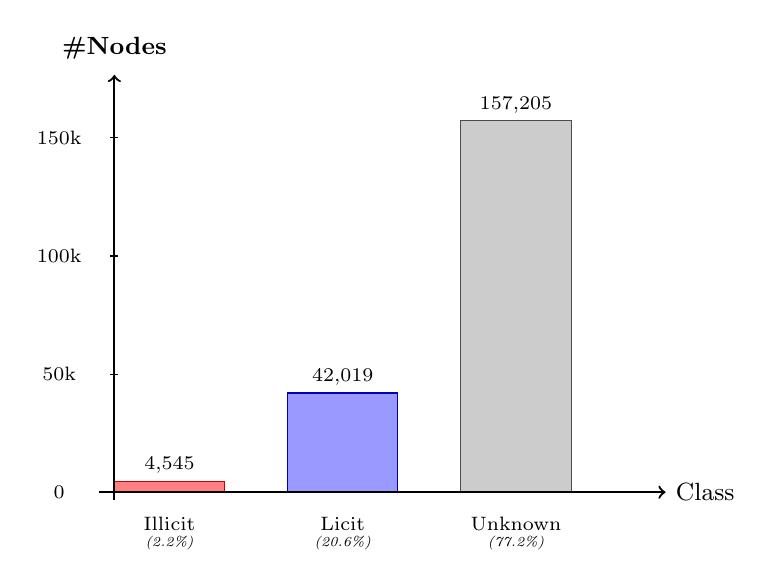
\begin{tikzpicture}[yscale=1.0]
% Bar chart: class distribution (hardcoded bar heights)
% Illicit: 4545 -> 0.137cm; Licit: 42019 -> 1.26cm; Unknown: 157205 -> 4.72cm
% Scale: 1 node = 0.00003 cm (157205 * 0.00003 = 4.72)

% Bars (hardcoded heights)
\fill[red!50!white, draw=red!80!black] (0.0,0) rectangle (1.4, 0.14);
\fill[blue!40!white, draw=blue!70!black] (2.2,0) rectangle (3.6, 1.26);
\fill[gray!40!white, draw=gray!60!black] (4.4,0) rectangle (5.8, 4.72);

% Labels on top of bars
\node at (0.7, 0.34) [font=\scriptsize] {4,545};
\node at (2.9, 1.46) [font=\scriptsize] {42,019};
\node at (5.1, 4.92) [font=\scriptsize] {157,205};

% Percentage labels
\node at (0.7, -0.4) [font=\scriptsize] {Illicit};
\node at (0.7, -0.65) [font=\tiny\itshape] {(2.2\%)};
\node at (2.9, -0.4) [font=\scriptsize] {Licit};
\node at (2.9, -0.65) [font=\tiny\itshape] {(20.6\%)};
\node at (5.1, -0.4) [font=\scriptsize] {Unknown};
\node at (5.1, -0.65) [font=\tiny\itshape] {(77.2\%)};

% Axes
\draw[->, thick] (-0.2, 0) -- (7.0, 0) node[right, font=\small] {Class};
\draw[->, thick] (0, -0.1) -- (0, 5.3) node[above=2pt, font=\small\bfseries] {\#Nodes};

% Y-axis ticks
\draw (0.05,0) -- (-0.05,0); \node at (-0.7,0) [font=\scriptsize] {0};
\draw (0.05,1.5) -- (-0.05,1.5); \node at (-0.7,1.5) [font=\scriptsize] {50k};
\draw (0.05,3.0) -- (-0.05,3.0); \node at (-0.7,3.0) [font=\scriptsize] {100k};
\draw (0.05,4.5) -- (-0.05,4.5); \node at (-0.7,4.5) [font=\scriptsize] {150k};
\end{tikzpicture}
\caption[Class Distribution in Elliptic Dataset]{Class distribution across all 203,769 transaction nodes in the Elliptic Bitcoin Dataset. The illicit class (4,545 nodes, 2.2\%) is severely under-represented relative to the licit (42,019) and unknown (157,205) classes, necessitating class-weighted loss functions.}
\label{fig:class_dist}
\end{figure}

Figure~\ref{fig:temporal_dist} shows the approximate distribution of nodes across the 49 time steps.

\begin{figure}[!htbp]
\centering
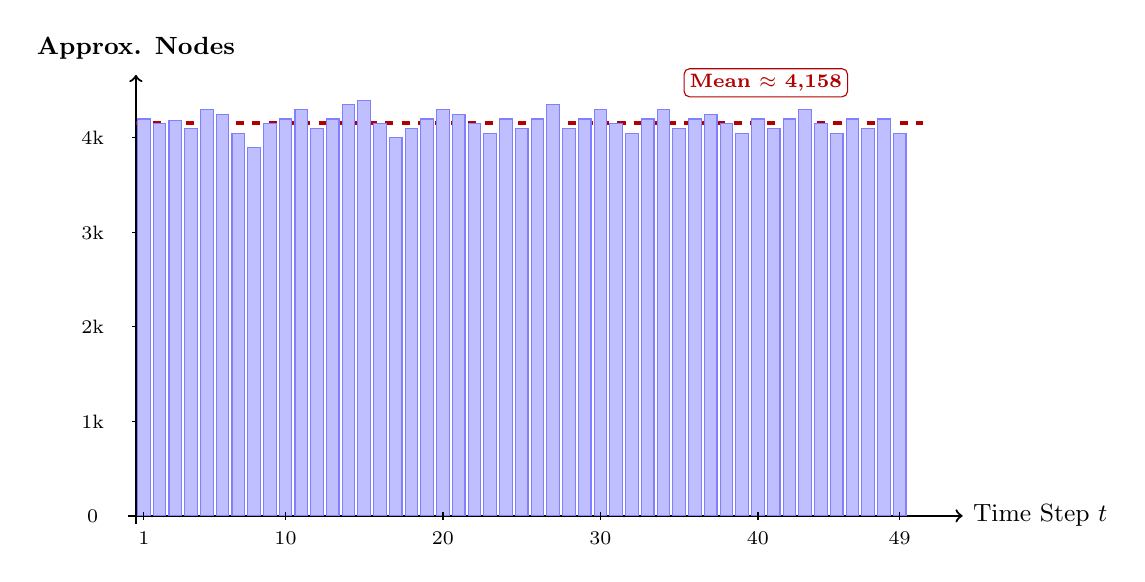
\begin{tikzpicture}
% Temporal distribution: 49 bars at ~4158 average
% Scale: 5000 nodes -> 5.0cm; each bar width = 0.16cm; spacing = 0.20cm total
% Bars represented at unit intervals; each time step bar colour uniform blue

% Axes
\draw[->, thick] (-0.1, 0) -- (10.5, 0) node[right, font=\small] {Time Step $t$};
\draw[->, thick] (0, -0.1) -- (0, 5.6) node[above=2pt, font=\small\bfseries] {Approx. Nodes};

% Y ticks
\draw (0.05,0) -- (-0.05,0); \node[font=\scriptsize] at (-0.55,0) {0};
\draw (0.05,1.2) -- (-0.05,1.2); \node[font=\scriptsize] at (-0.55,1.2) {1k};
\draw (0.05,2.4) -- (-0.05,2.4); \node[font=\scriptsize] at (-0.55,2.4) {2k};
\draw (0.05,3.6) -- (-0.05,3.6); \node[font=\scriptsize] at (-0.55,3.6) {3k};
\draw (0.05,4.8) -- (-0.05,4.8); \node[font=\scriptsize] at (-0.55,4.8) {4k};

% Mean line at 4158 nodes -> 4158/1000 * 1.2 = 4.99
\draw[dashed, ultra thick, red!70!black] (0, 4.99) -- (10.0, 4.99);
\node at (8.0, 5.5) [font=\scriptsize\bfseries, text=red!70!black, fill=white, draw=red!70!black, rounded corners=2pt, inner sep=2pt] {Mean $\approx$ 4,158};

% 49 bars, each 0.18cm wide, spaced 0.20cm apart, heights ~5cm (varying slightly)
% Heights in cm (representing ~4000-4400 nodes, scale: 1k nodes = 1.2cm)
\foreach \i/\hi in {
  1/5.04, 2/4.98, 3/5.02, 4/4.92, 5/5.16, 6/5.10, 7/4.86, 8/4.68,
  9/4.98, 10/5.04, 11/5.16, 12/4.92, 13/5.04, 14/5.22, 15/5.28, 16/4.98,
  17/4.80, 18/4.92, 19/5.04, 20/5.16, 21/5.10, 22/4.98, 23/4.86, 24/5.04,
  25/4.92, 26/5.04, 27/5.22, 28/4.92, 29/5.04, 30/5.16, 31/4.98, 32/4.86,
  33/5.04, 34/5.16, 35/4.92, 36/5.04, 37/5.10, 38/4.98, 39/4.86, 40/5.04,
  41/4.92, 42/5.04, 43/5.16, 44/4.98, 45/4.86, 46/5.04, 47/4.92, 48/5.04, 49/4.86
}{
  \pgfmathsetmacro\xpos{(\i-1)*0.20 + 0.10}
  \fill[blue!25, draw=blue!50] (\xpos-0.08, 0) rectangle (\xpos+0.08, \hi);
}

% X ticks
\foreach \t/\xpos in {1/0.10, 10/1.90, 20/3.90, 30/5.90, 40/7.90, 49/9.70}{
  \draw (\xpos, 0.05) -- (\xpos, -0.05);
  \node[font=\scriptsize] at (\xpos, -0.28) {\t};
}
\end{tikzpicture}
\caption[Temporal Distribution of Transactions]{Approximate distribution of transaction nodes across the 49 time steps of the Elliptic Bitcoin Dataset. The red dashed line indicates the mean of approximately 4,158 nodes per time step. Values are representative approximations; exact per-step counts require computation from the raw dataset.}
\label{fig:temporal_dist}
\end{figure}


---

\section{Algorithm and Model Design}
\label{sec:algo_design}

\subsection{Objective 1 — Temporal Graph Construction}
\label{subsec:graph_construction}

Figure~\ref{fig:graph_construction} illustrates the temporal graph construction workflow.

\begin{figure}[!htbp]
\centering
\begin{tikzpicture}[
    flowstep/.style={rectangle, draw=black, fill=yellow!10, rounded corners=3pt, thick,
                 text width=9.5cm, minimum height=0.9cm, align=left, font=\small},
    arrow/.style={->, >=stealth, thick, draw=gray!70},
]
\node[flowstep, fill=gray!10] (s1)
  {\textbf{Step 1:} Load 3 Elliptic CSV files (features, edgelist, classes).};
\node[flowstep, below=0.3cm of s1, fill=yellow!10] (s2)
  {\textbf{Step 2:} Remap txId $\in \mathbb{Z}^+$ to contiguous indices $[0, 203768]$ via hash map.};
\node[flowstep, below=0.3cm of s2] (s3)
  {\textbf{Step 3:} Construct directed edge index tensor $\mathbf{E} \in \mathbb{Z}^{2 \times 234355}$.};
\node[flowstep, below=0.3cm of s3, fill=blue!8] (s4)
  {\textbf{Step 4:} Engineer 6 topological features; concatenate to obtain $\mathbf{X} \in \mathbb{R}^{203769 \times 172}$.};
\node[flowstep, below=0.3cm of s4, fill=green!8] (s5)
  {\textbf{Step 5:} Fit StandardScaler on training nodes ($t \leq 34$); transform all nodes.};
\node[flowstep, below=0.3cm of s5, fill=orange!8] (s6)
  {\textbf{Step 6:} Assign chronological split masks (train / val / test). Assemble PyG Data object.};

\draw[arrow] (s1) -- (s2);
\draw[arrow] (s2) -- (s3);
\draw[arrow] (s3) -- (s4);
\draw[arrow] (s4) -- (s5);
\draw[arrow] (s5) -- (s6);
\end{tikzpicture}
\caption[Temporal Graph Construction Workflow]{Step-by-step workflow for constructing the temporal graph from the Elliptic Bitcoin Dataset.}
\label{fig:graph_construction}
\end{figure}

\noindent \textbf{Engineered Topological Features:} In addition to the raw 166 dataset features, six domain-specific topological features are engineered to provide immediate structural signals relevant to AML. Table~\ref{tab:engineered_features} defines each feature.

\begin{table}[!htbp]
\centering
\caption[Engineered Topological Features]{Six engineered topological features appended to each transaction node, expanding the feature dimension from 166 to 172.}
\label{tab:engineered_features}
\begin{tabularx}{\textwidth}{>{\hsize=0.85\hsize}L >{\hsize=1.0\hsize}L >{\hsize=1.15\hsize}L}
\toprule
\textbf{Feature} & \textbf{Mathematical Definition} & \textbf{AML Rationale} \\
\midrule
Out-Degree ($d_{\text{out}}$) & $\sum_{(v, u) \in E} 1$ & Identifies fund-dispersal nodes (smurfing originators). \\
In-Degree ($d_{\text{in}}$) & $\sum_{(u, v) \in E} 1$ & Identifies fund-aggregation nodes (smurfing collection points). \\
Fan-Out Ratio & $\dfrac{d_{\text{out}}}{d_{\text{in}} + d_{\text{out}} + \epsilon}$ & High ratio ($> 0.8$) signifies fund dispersal phase. \\
Fan-In Ratio & $\dfrac{d_{\text{in}}}{d_{\text{in}} + d_{\text{out}} + \epsilon}$ & High ratio ($> 0.8$) signifies fund aggregation phase. \\
Temporal Recency & $t_v / 49.0$ & Continuous temporal position of transaction in $[0, 1]$. \\
Neighbour Time Delta & $\frac{1}{|\mathcal{N}(v)|} \sum_{u \in \mathcal{N}(v)} |t_v - t_u|$ & Measures transaction velocity and dormancy duration. \\
\bottomrule
\end{tabularx}
\end{table}

\noindent \textbf{Mathematical Formulation:}
\begin{equation}
\mathbf{X}^{(172)} = \left[ \mathbf{X}^{(166)}_{\text{raw}} \;\big\|\; d_{\text{out}}, \; d_{\text{in}}, \; r_{\text{out}}, \; r_{\text{in}}, \; \frac{t_v}{49}, \; \bar{\delta}_{\mathcal{N}(v)} \right]
\label{eq:feature_expansion}
\end{equation}

Figure~\ref{fig:graph_representation} illustrates the temporal graph with nodes, directed edges, and time step labels.

\begin{figure}[!htbp]
\centering
\begin{tikzpicture}[
    tnode/.style={circle, draw=black, fill=blue!12, thick, minimum size=1.0cm, font=\small},
    inode/.style={circle, draw=red!80!black, fill=red!15, thick, minimum size=1.0cm, font=\small},
    edge/.style={->, >=stealth, thick, draw=gray!70},
    iedge/.style={->, >=stealth, thick, draw=red!60},
    tlabel/.style={font=\scriptsize, text=gray!85!black, fill=white, inner sep=1.5pt, rounded corners=1pt},
]
\node[tnode, label=left:{\tiny $t=5$}] (n1) at (0, 0) {$v_1$};
\node[tnode, label=above:{\tiny $t=7$}] (n2) at (2.5, 1.2) {$v_2$};
\node[inode, label=above:{\tiny $t=8$}] (n3) at (5.0, 1.2) {$v_3$};
\node[tnode, label=below:{\tiny $t=9$}] (n4) at (2.5,-1.2) {$v_4$};
\node[inode, label=right:{\tiny $t=12$}] (n5) at (7.5, 0) {$v_5$};

\draw[edge] (n1) -- (n2) node[midway, above, tlabel] {$\Delta t=2$};
\draw[edge] (n1) -- (n4) node[midway, below, tlabel] {$\Delta t=4$};
\draw[iedge] (n2) -- (n3) node[midway, above, tlabel] {$\Delta t=1$};
\draw[iedge] (n3) -- (n5) node[midway, above, tlabel] {$\Delta t=4$};
\draw[edge] (n4) -- (n5) node[midway, below, tlabel] {$\Delta t=3$};

% Legend
\node[tnode, minimum size=0.6cm, right=0.5cm of n5, yshift=0.5cm] (ll) {};
\node[right=0.1cm of ll, font=\tiny] {Licit};
\node[inode, minimum size=0.6cm, right=0.5cm of n5, yshift=-0.5cm] (li) {};
\node[right=0.1cm of li, font=\tiny] {Illicit};
\end{tikzpicture}
\caption[Temporal Graph Representation]{Illustration of the temporal graph $G = (V, E, \mathbf{X}, \mathbf{T})$. Each node $v_i$ is labelled with its time step $t$. Directed edges show UTXO fund flows, with $\Delta t$ labels indicating the time difference between connected transactions. Blue nodes are licit; red nodes are illicit.}
\label{fig:graph_representation}
\end{figure}

\subsection{Objective 2 — Learnable Fourier Time Encoding}
\label{subsec:fourier_encoding}

This subsection describes the core technical novelty of TemporalAML: a trainable Fourier time encoding module integrated directly into the graph attention mechanism.

\vspace{0.5em}
\noindent \textbf{Motivation:} Standard TGAT~\cite{xu2020tgat} uses fixed sinusoidal frequencies calibrated for NLP token sequences:
\begin{equation}
\omega_k^{\text{fixed}} = 10000^{-2k/d}, \quad k = 1, 2, \ldots, d/2
\label{eq:fixed_freq}
\end{equation}
Cryptocurrency transaction intervals are non-stationary and bursty (following a power-law distribution). Fixed frequencies cannot adapt to the specific time scales of rapid layering hops (minutes) or slow dormancy cycles (weeks). TemporalAML replaces fixed frequencies with \textbf{trainable parameters learned by gradient descent}.

\vspace{0.5em}
\noindent \textbf{Theoretical Foundation:} By Bochner's Theorem~\cite{bochner1933monotone}, any continuous, shift-invariant kernel $K(\Delta t) = \psi(t_i - t_j)$ can be expressed as the Fourier transform of a positive measure. This justifies representing temporal similarity through a sum of complex exponentials (equivalently, sin/cos pairs).

\vspace{0.5em}
\noindent \textbf{Learnable Fourier Time Encoding Formula:}
\begin{equation}
\Phi(\Delta t) = \sqrt{\frac{1}{k}} \Big[ \cos(\omega_1 \Delta t + \phi_1), \; \sin(\omega_1 \Delta t + \phi_1), \; \ldots, \; \cos(\omega_k \Delta t + \phi_k), \; \sin(\omega_k \Delta t + \phi_k) \Big]
\label{eq:fourier_encoding}
\end{equation}
where:
\begin{itemize}
	\item $\Delta t = t_{\text{target}} - t_{\text{source}} \geq 0$ is the continuous edge time delta.
	\item $k = 64$ is the number of frequency components; the output dimension is $d_t = 2k = 128$.
	\item $\boldsymbol{\omega} \in \mathbb{R}^{k}$ are \textbf{learnable frequency parameters}, initialised from $\mathcal{N}(0, 0.01)$.
	\item $\boldsymbol{\phi} \in \mathbb{R}^{k}$ are \textbf{learnable phase shift parameters}, initialised to zero.
	\item $\sqrt{1/k}$ is a normalisation scalar.
\end{itemize}

\vspace{0.5em}
\noindent \textbf{Learnability via Gradient Descent:} The gradient of the encoding with respect to frequency parameter $\omega_j$ is:
\begin{equation}
\frac{\partial \Phi_j(\Delta t)}{\partial \omega_j} = -\Delta t \cdot \sin(\omega_j \Delta t + \phi_j) \neq 0
\label{eq:fourier_gradient}
\end{equation}
Since this gradient is non-zero for almost all $\Delta t > 0$, the loss gradient $\frac{\partial \mathcal{L}}{\partial \boldsymbol{\omega}} = \frac{\partial \mathcal{L}}{\partial \Phi} \cdot \frac{\partial \Phi}{\partial \boldsymbol{\omega}}$ flows back to dynamically calibrate frequencies to the characteristic velocity of cryptocurrency laundering hops.

Figure~\ref{fig:fourier_arch} shows the Fourier Time Encoding architecture.

\begin{figure}[!htbp]
\centering
\begin{tikzpicture}[
    block/.style={rectangle, draw=blue!60!black, fill=blue!8, rounded corners=3pt, thick,
                  text width=5.2cm, minimum height=0.75cm, align=center, font=\small},
    param/.style={rectangle, draw=orange!80!black, fill=orange!12, rounded corners=3pt, thick,
                  text width=4.6cm, minimum height=0.75cm, align=center, font=\small},
    arrow/.style={->, >=stealth, thick, draw=gray!70},
    concat/.style={rectangle, draw=green!60!black, fill=green!8, rounded corners=3pt, thick,
                   text width=5.2cm, minimum height=0.75cm, align=center, font=\small},
]
\node[block] (dt) {Time Delta $\Delta t = t_i - t_j$};
\node[param, below=0.6cm of dt, xshift=-3.0cm] (omega) {Learnable $\boldsymbol{\omega} \in \mathbb{R}^{64}$ (Frequencies)};
\node[param, below=0.6cm of dt, xshift=3.0cm] (phi) {Learnable $\boldsymbol{\phi} \in \mathbb{R}^{64}$ (Phases)};
\node[block, below=0.7cm of omega] (cos) {$\cos(\boldsymbol{\omega}\Delta t + \boldsymbol{\phi})$};
\node[block, below=0.7cm of phi] (sin) {$\sin(\boldsymbol{\omega}\Delta t + \boldsymbol{\phi})$};
\node[concat, below=0.7cm of $(cos)!0.5!(sin)$] (cat) {Concatenate: $[\cos \;\|\; \sin] \in \mathbb{R}^{128}$};
\node[block, below=0.5cm of cat, fill=green!15, draw=green!60!black] (norm) {Scale $\times \sqrt{1/64}$ $\Rightarrow$ $\Phi(\Delta t) \in \mathbb{R}^{128}$};

\draw[arrow] (dt.south) -- ++(0,-0.2) -| (cos.north);
\draw[arrow] (dt.south) -- ++(0,-0.2) -| (sin.north);
\draw[arrow] (omega) -- (cos);
\draw[arrow] (phi) -- (sin);
\draw[arrow] (cos) -- (cat);
\draw[arrow] (sin) -- (cat);
\draw[arrow] (cat) -- (norm);
\end{tikzpicture}
\caption[Learnable Fourier Time Encoding Architecture]{Architecture of the Learnable Fourier Time Encoding module. The time delta $\Delta t$ is multiplied with trainable frequency parameters $\boldsymbol{\omega}$ and summed with trainable phase shifts $\boldsymbol{\phi}$, projected through cosine and sine functions, concatenated, and normalised to produce a 128-dimensional temporal embedding $\Phi(\Delta t)$.}
\label{fig:fourier_arch}
\end{figure}

\subsection{Objective 3 — Temporal Graph Attention Network (TGAT)}
\label{subsec:tgat}

\subsubsection{Temporal Neighbourhood and Causal Masking}

For each target node $v_i$ with time step $t_i$, the causal temporal neighbourhood is defined as:
\begin{equation}
\mathcal{N}_{\text{causal}}(v_i) = \{ v_j \in \mathcal{N}(v_i) \mid t_j \leq t_i \}
\label{eq:causal_neighborhood}
\end{equation}
This ensures that the attention mechanism only aggregates information from transactions occurring \textit{at or before} the target transaction, preventing future data leakage during both training and inference.

\subsubsection{TGAT Layer Computation}

Each TGATConv layer computes temporally-aware node representations through a query-key-value attention mechanism. Let $\mathbf{h}_i^{(l)}$ denote the node $i$ representation at layer $l$:

\begin{equation}
\mathbf{q}_i = \left[\mathbf{h}_i^{(l)} \;\big\|\; \Phi(0)\right] \mathbf{W}_Q
\label{eq:query}
\end{equation}

\begin{equation}
\mathbf{k}_j = \left[\mathbf{h}_j^{(l)} \;\big\|\; \Phi(t_i - t_j)\right] \mathbf{W}_K, \qquad \mathbf{v}_j = \left[\mathbf{h}_j^{(l)} \;\big\|\; \Phi(t_i - t_j)\right] \mathbf{W}_V
\label{eq:key_value}
\end{equation}

\begin{equation}
\alpha_{ij} = \text{softmax}\left( \frac{\mathbf{q}_i \mathbf{k}_j^\top}{\sqrt{d_k}} \right) = \frac{\exp\!\left( \frac{\mathbf{q}_i \mathbf{k}_j^\top}{\sqrt{d_k}} \right)}{\sum_{u \in \mathcal{N}_{\text{causal}}(i)} \exp\!\left( \frac{\mathbf{q}_i \mathbf{k}_u^\top}{\sqrt{d_k}} \right)}
\label{eq:attention}
\end{equation}

\begin{equation}
\mathbf{h}_i^{(l+1)} = \text{LayerNorm}\!\left( \sum_{j \in \mathcal{N}_{\text{causal}}(i)} \alpha_{ij} \mathbf{v}_j \;+\; \mathbf{W}_{\text{res}} \mathbf{h}_i^{(l)} \right)
\label{eq:tgat_update}
\end{equation}

\noindent where $\mathbf{W}_Q, \mathbf{W}_K, \mathbf{W}_V \in \mathbb{R}^{(d_h + d_t) \times d_k}$ are learnable projection matrices, $d_h = 128$ is the node embedding dimension, $d_t = 128$ is the Fourier encoding dimension, $d_k = 64$ is the attention head dimension, and $\mathbf{W}_{\text{res}}$ is the residual projection matrix.

Figure~\ref{fig:tgat_arch} illustrates the complete TGAT layer architecture.

\begin{figure}[!htbp]
\centering
\begin{tikzpicture}[
    block/.style={rectangle, draw=black, fill=blue!8, rounded corners=3pt, thick,
                  minimum width=3.5cm, minimum height=0.9cm, align=center, font=\small},
    arrow/.style={->, >=stealth, thick, draw=gray!70},
    label/.style={font=\scriptsize\itshape, text=gray!70},
]
% Input row
\node[block, fill=gray!10] (xi) at (0,0) {$\mathbf{h}_i^{(l)}$ (target)};
\node[block, fill=gray!10] (xj) at (5,0) {$\mathbf{h}_j^{(l)}$ (neighbour)};
\node[block, fill=orange!10] (phi) at (5,-1.5) {$\Phi(t_i - t_j)$ (Fourier encoding)};

% Concat
\node[block, fill=blue!10] (concatq) at (0,-1.5) {$[\mathbf{h}_i \| \Phi(0)]$};
\node[block, fill=blue!10] (concatk) at (5,-3.0) {$[\mathbf{h}_j \| \Phi(\Delta t)]$};

% QKV
\node[block, fill=green!10] (q) at (0,-3.0) {$\mathbf{q}_i = [\cdot]\mathbf{W}_Q$};
\node[block, fill=green!10] (k) at (5,-4.5) {$\mathbf{k}_j = [\cdot]\mathbf{W}_K$};
\node[block, fill=green!10] (v) at (9,-4.5) {$\mathbf{v}_j = [\cdot]\mathbf{W}_V$};

% Attention
\node[block, fill=yellow!15] (attn) at (2.5,-5.5) {$\alpha_{ij} = \text{softmax}\!\left(\dfrac{\mathbf{q}_i\mathbf{k}_j^\top}{\sqrt{d_k}}\right)$};

% Aggregation
\node[block, fill=red!8] (agg) at (5.5,-7.0) {$\sum_{j} \alpha_{ij}\mathbf{v}_j$ + Residual};
\node[block, fill=blue!12] (out) at (5.5,-8.2) {LayerNorm $\Rightarrow$ $\mathbf{h}_i^{(l+1)} \in \mathbb{R}^{128}$};

% Arrows
\draw[arrow] (xi) -- (concatq);
\draw[arrow] (concatq) -- (q);
\draw[arrow] (xj) -- (concatk);
\draw[arrow] (phi) -- (concatk);
\draw[arrow] (concatk) -- (k);
\draw[arrow] (concatk) -- (v);
\draw[arrow] (q) -- (attn);
\draw[arrow] (k) -- (attn);
\draw[arrow] (attn) -- (agg);
\draw[arrow] (v) -- (agg);
\draw[arrow] (agg) -- (out);
\end{tikzpicture}
\caption[TGAT Layer Architecture]{Architecture of a single Temporal Graph Attention (TGAT) layer. The target node $v_i$ and each causal neighbour $v_j$ are concatenated with their respective Fourier time encodings ($\Phi(0)$ for the target and $\Phi(t_i - t_j)$ for the neighbour) before attention projection. The attention coefficient $\alpha_{ij}$ modulates the aggregation of neighbour value vectors, with a residual connection and layer normalisation.}
\label{fig:tgat_arch}
\end{figure}

\subsubsection{Multi-Pattern AML Detection Heads}
\label{subsubsec:pattern_heads}

The two-layer TGATConv encoder produces a shared 128-dimensional latent embedding $\mathbf{Z} \in \mathbb{R}^{N \times 128}$ for all nodes. Three parallel feed-forward classification heads operate on these shared embeddings:

\begin{align}
\hat{y}^{\text{circ}}_v &= \sigma\!\left( \mathbf{W}^{\text{circ}}_2 \;\text{ReLU}\!\left(\mathbf{W}^{\text{circ}}_1 \mathbf{z}_v + \mathbf{b}^{\text{circ}}_1\right) + \mathbf{b}^{\text{circ}}_2 \right) \label{eq:circ_head} \\
\hat{y}^{\text{lay}}_v &= \sigma\!\left( \mathbf{W}^{\text{lay}}_2 \;\text{ReLU}\!\left(\mathbf{W}^{\text{lay}}_1 \mathbf{z}_v + \mathbf{b}^{\text{lay}}_1\right) + \mathbf{b}^{\text{lay}}_2 \right) \label{eq:lay_head} \\
\hat{y}^{\text{smurf}}_v &= \sigma\!\left( \mathbf{W}^{\text{smurf}}_2 \;\text{ReLU}\!\left(\mathbf{W}^{\text{smurf}}_1 \mathbf{z}_v + \mathbf{b}^{\text{smurf}}_1\right) + \mathbf{b}^{\text{smurf}}_2 \right) \label{eq:smurf_head}
\end{align}

where $\sigma$ denotes the sigmoid activation function and $\mathbf{z}_v \in \mathbb{R}^{128}$ is the shared TGAT node embedding.

\vspace{0.5em}
\noindent \textbf{Joint Multi-Task Loss:}
\begin{equation}
\begin{split}
\mathcal{L}_{\text{total}} = {} & \lambda_1 \;\text{WBCE}(\hat{y}^{\text{circ}}, y^{\text{circ}}, w_1) + \lambda_2 \;\text{WBCE}(\hat{y}^{\text{lay}}, y^{\text{lay}}, w_2) \\
& + \lambda_3 \;\text{WBCE}(\hat{y}^{\text{smurf}}, y^{\text{smurf}}, w_3)
\end{split}
\label{eq:joint_loss}
\end{equation}
where $\text{WBCE}$ is the Weighted Binary Cross-Entropy loss, $w_k = N_{\text{neg},k} / N_{\text{pos},k}$ is the positive-class weight for pattern $k$ to mitigate class imbalance, and $\lambda_1 = \lambda_2 = \lambda_3 = 1.0$.

\vspace{0.5em}
\noindent \textbf{Ground-Truth Pattern Label Mining:} Because the Elliptic dataset provides only binary illicit/licit labels, pattern-specific ground-truth labels are mined algorithmically from the graph topology:
\begin{itemize}
	\item $y^{\text{circ}} = 1$ for illicit nodes participating in a Strongly Connected Component (SCC) of size $\geq 2$, computed using Tarjan's SCC algorithm.
	\item $y^{\text{lay}} = 1$ for illicit nodes on directed paths of length $\geq 3$ with monotonically increasing timestamps ($t_{k+1} \geq t_k$), identified by temporal directed BFS.
	\item $y^{\text{smurf}} = 1$ for illicit nodes with out-degree $d_{\text{out}} \geq 10$ or in-degree $d_{\text{in}} \geq 10$.
\end{itemize}

\noindent \textbf{Domain Constraint Note:} The Bitcoin UTXO model is a strict Directed Acyclic Graph at the transaction level—transaction outputs cannot be consumed by ancestor transactions. Consequently, closed transaction-level cycles ($A \to B \to C \to A$) cannot exist in the raw Elliptic transaction graph. Circular transfer detection is therefore architecturally included for completeness and future applicability to wallet-entity-level graphs, while the primary pattern signals in the current framework are Layering Chains and Smurfing.

\vspace{1em}
\noindent Figures~\ref{fig:circular_pattern}, \ref{fig:layering_pattern}, and \ref{fig:smurfing_pattern} illustrate the three targeted laundering patterns.

\begin{figure}[!htbp]
\centering
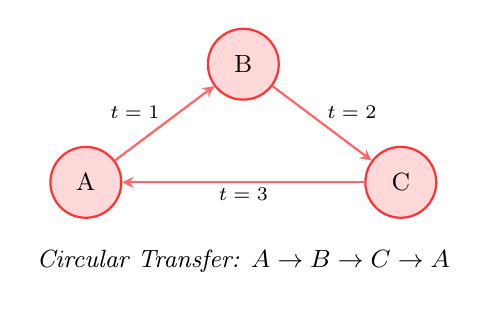
\begin{tikzpicture}[
    wnode/.style={circle, draw=red!80, fill=red!15, thick, minimum size=0.9cm, font=\small},
    edge/.style={->, >=stealth, thick, draw=red!60},
]
\node[wnode] (A) at (0,0) {A};
\node[wnode] (B) at (2,1.5) {B};
\node[wnode] (C) at (4,0) {C};
\draw[edge] (A) -- (B) node[midway, above left, font=\scriptsize, fill=white, inner sep=1.5pt, rounded corners=1pt] {$t=1$};
\draw[edge] (B) -- (C) node[midway, above right, font=\scriptsize, fill=white, inner sep=1.5pt, rounded corners=1pt] {$t=2$};
\draw[edge] (C) -- (A) node[midway, below, font=\scriptsize, fill=white, inner sep=1.5pt, rounded corners=1pt] {$t=3$};
\node at (2, -1.0) [font=\small\itshape] {Circular Transfer: $A \to B \to C \to A$};
\end{tikzpicture}
\caption[Circular Transfer Pattern]{Circular Transfer pattern: funds cycle through a closed loop ($A \to B \to C \to A$) to simulate wash trading, confuse audit tracing systems, and obscure the origin of illicit proceeds. Detected via Tarjan's Strongly Connected Components algorithm.}
\label{fig:circular_pattern}
\end{figure}

\begin{figure}[!htbp]
\centering
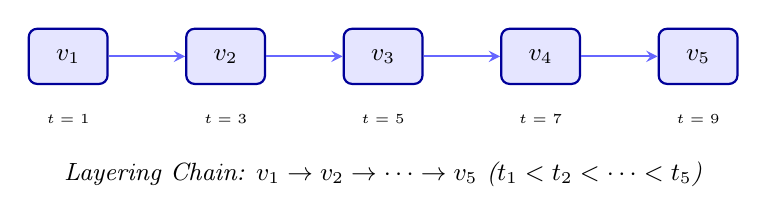
\begin{tikzpicture}[
    wnode/.style={rectangle, draw=blue!60!black, fill=blue!10, thick, rounded corners=3pt, minimum width=1.0cm, minimum height=0.7cm, font=\small},
    edge/.style={->, >=stealth, thick, draw=blue!60},
]
\node[wnode] (n1) at (0,0) {$v_1$};
\node[wnode] (n2) at (2,0) {$v_2$};
\node[wnode] (n3) at (4,0) {$v_3$};
\node[wnode] (n4) at (6,0) {$v_4$};
\node[wnode] (n5) at (8,0) {$v_5$};
\node at (0,-0.8) [font=\tiny\itshape] {$t=1$};
\node at (2,-0.8) [font=\tiny\itshape] {$t=3$};
\node at (4,-0.8) [font=\tiny\itshape] {$t=5$};
\node at (6,-0.8) [font=\tiny\itshape] {$t=7$};
\node at (8,-0.8) [font=\tiny\itshape] {$t=9$};
\draw[edge] (n1) -- (n2);
\draw[edge] (n2) -- (n3);
\draw[edge] (n3) -- (n4);
\draw[edge] (n4) -- (n5);
\node at (4,-1.5) [font=\small\itshape] {Layering Chain: $v_1 \to v_2 \to \cdots \to v_5$ ($t_1 < t_2 < \cdots < t_5$)};
\end{tikzpicture}
\caption[Layering Chain Pattern]{Layering Chain pattern: funds are forwarded across a linear sequence of transaction hops with monotonically increasing timestamps ($t_1 < t_2 < \ldots < t_k$, $k \geq 3$). Rapid layering exploits hop-decay AML heuristics. Detected via temporal directed BFS.}
\label{fig:layering_pattern}
\end{figure}

\begin{figure}[!htbp]
\centering
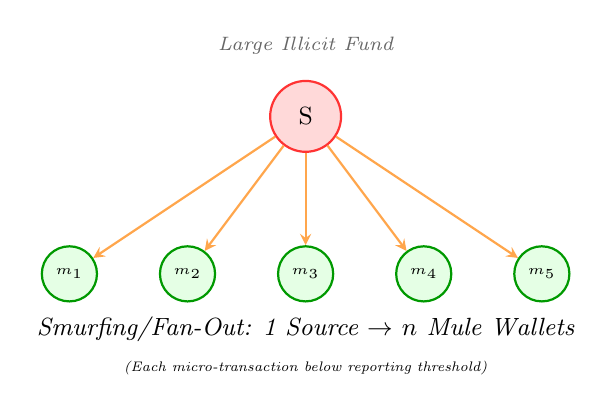
\begin{tikzpicture}[
    source/.style={circle, draw=red!80, fill=red!15, thick, minimum size=0.9cm, font=\small},
    mule/.style={circle, draw=green!60!black, fill=green!10, thick, minimum size=0.7cm, font=\tiny},
    edge/.style={->, >=stealth, thick, draw=orange!70},
]
\node[source] (S) at (3,0) {S};
\node[mule] (m1) at (0,-2) {$m_1$};
\node[mule] (m2) at (1.5,-2) {$m_2$};
\node[mule] (m3) at (3,-2) {$m_3$};
\node[mule] (m4) at (4.5,-2) {$m_4$};
\node[mule] (m5) at (6,-2) {$m_5$};
\draw[edge] (S) -- (m1);
\draw[edge] (S) -- (m2);
\draw[edge] (S) -- (m3);
\draw[edge] (S) -- (m4);
\draw[edge] (S) -- (m5);
\node at (3, 0.9) [font=\scriptsize\itshape, text=gray!80!black] {Large Illicit Fund};
\node at (3,-2.7) [font=\small\itshape] {Smurfing/Fan-Out: 1 Source $\to$ $n$ Mule Wallets};
\node at (3,-3.2) [font=\tiny\itshape] {(Each micro-transaction below reporting threshold)};
\end{tikzpicture}
\caption[Smurfing / Fan-Out Pattern]{Smurfing (Fan-Out / Structuring) pattern: a single source transaction splits a large illicit fund into multiple micro-transactions directed to many destination mule wallets, each below mandatory reporting thresholds (e.g., \$10,000 FATF limit). Detected by degree thresholding ($d_{\text{out}} \geq 10$).}
\label{fig:smurfing_pattern}
\end{figure}

\subsection{Objective 4 — Per-Pattern Subgraph Explainability}
\label{subsec:explainability}

\subsubsection{Why Explainability is Necessary in AML}

Financial regulators (FATF, FinCEN, FCA) require AML alerts to be accompanied by auditable evidence trails sufficient to support Suspicious Activity Report (SAR) filing. A scalar probability score alone is not actionable: compliance officers need to know \textit{which specific transactions} formed the suspicious pattern and \textit{in what temporal order} funds flowed through the network.

\subsubsection{GNNExplainer}

GNNExplainer~\cite{ying2019gnnexplainer} is a model-agnostic post-hoc explainability method that, given a trained GNN and a target node $v^*$, learns a soft edge mask $\mathbf{M} \in [0,1]^{|E_{s}|}$ by solving the following mutual information maximisation problem:
\begin{equation}
\max_{\mathbf{M}} \; \text{MI}\!\left( Y_{v^*}^G, \; Y_{v^*}^{G_s} \right) = H\!\left(Y_{v^*}^G\right) - H\!\left(Y_{v^*}^G \mid G_s = (A \odot \sigma(\mathbf{M}), \mathbf{X})\right)
\label{eq:gnnexplainer}
\end{equation}
where $Y_{v^*}^G$ is the model's prediction on the full graph, $G_s$ is the masked subgraph, $\odot$ is element-wise multiplication, and $H(\cdot)$ is the Shannon entropy. The optimisation is performed by gradient ascent on $\mathbf{M}$ for a fixed number of epochs (typically 200), after which a threshold is applied to select the top-$k$ most important edges.

\subsubsection{Per-Pattern Evidence Generation}

For each flagged alert node $v^*$:
\begin{enumerate}
	\item GNNExplainer is activated independently for each positive pattern head (e.g., if $\hat{y}^{\text{lay}}_{v^*} > 0.5$, the layering head's prediction is explained).
	\item The optimised edge mask $\mathbf{M}^*$ identifies the $k$ most important transaction edges contributing to the pattern classification.
	\item These edges, along with their associated nodes and timestamps, are extracted to form the \textit{evidence subgraph} $G_s$.
	\item The evidence subgraph nodes are sorted by timestamp to generate a \textit{time-ordered transaction chain}.
\end{enumerate}

Figure~\ref{fig:gnnexplainer_workflow} illustrates the GNNExplainer workflow.

\begin{figure}[!htbp]
\centering
\vspace{-0.5em}
\begin{tikzpicture}[
  block/.style={rectangle, draw=blue!60, fill=blue!5, very thick,
    text width=0.88\textwidth, align=left, rounded corners=3pt,
    font=\footnotesize, inner sep=2.5pt},
  arrow/.style={->, >=stealth, thick, color=blue!60}
]
\node[block, fill=red!8] (input)
  {\textbf{Input:} Flagged alert node $v^*$ with predicted probability $\hat{y}^{\text{lay}}_{v^*} > 0.5$};
\node[block, below=0.08cm of input, fill=orange!8] (freeze)
  {\textbf{Step 1:} Freeze trained TGAT weights; initialise edge mask $\mathbf{M} \in [0,1]^{|E_s|}$};
\node[block, below=0.08cm of freeze, fill=yellow!10] (optim)
  {\textbf{Step 2:} Gradient ascent on $\mathbf{M}$ (200 epochs) to maximise MI($Y^G_{v^*}, Y^{G_s}_{v^*}$)};
\node[block, below=0.08cm of optim, fill=green!8] (select)
  {\textbf{Step 3:} Threshold optimised mask $\mathbf{M}^*$; select top-$k$ causal edges and induced nodes};
\node[block, below=0.08cm of select, fill=blue!10] (sort)
  {\textbf{Step 4:} Sort selected nodes chronologically by timestamp ($t_1 \le t_2 \le \dots \le t^*$)};
\node[block, below=0.08cm of sort, fill=gray!10] (output)
  {\textbf{Output:} Evidence chain $G_s = \{v_1(t_1) \to \dots \to v^*(t^*)\}$ + Pattern Label + SAR narrative};

\draw[arrow] (input) -- (freeze);
\draw[arrow] (freeze) -- (optim);
\draw[arrow] (optim) -- (select);
\draw[arrow] (select) -- (sort);
\draw[arrow] (sort) -- (output);
\end{tikzpicture}
\vspace{-0.5em}
\caption[GNNExplainer Workflow]{Step-by-step GNNExplainer workflow for per-alert, per-pattern subgraph evidence generation in TemporalAML.}
\label{fig:gnnexplainer_workflow}
\end{figure}

Figure~\ref{fig:explainable_subgraph} illustrates a conceptual time-ordered explainable subgraph.

\begin{figure}[!htbp]
\centering
\vspace{-0.5em}
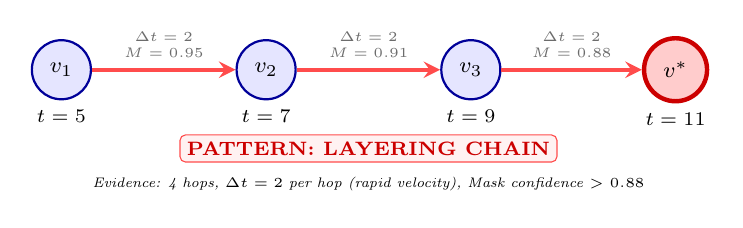
\begin{tikzpicture}[
    enode/.style={circle, draw=blue!60!black, fill=blue!10, thick, minimum size=0.75cm, font=\footnotesize},
    anode/.style={circle, draw=red!80!black, fill=red!20, ultra thick, minimum size=0.8cm, font=\footnotesize\bfseries},
    edge/.style={->, >=stealth, thick, draw=blue!60},
    hiledge/.style={->, >=stealth, ultra thick, draw=red!70},
    tlabel/.style={font=\tiny, text=gray!85!black, fill=white, inner sep=1.5pt, rounded corners=1pt, align=center},
]
\node[enode, label=below:{\scriptsize $t=5$}] (n1) at (0,0) {$v_1$};
\node[enode, label=below:{\scriptsize $t=7$}] (n2) at (2.6,0) {$v_2$};
\node[enode, label=below:{\scriptsize $t=9$}] (n3) at (5.2,0) {$v_3$};
\node[anode, label=below:{\scriptsize $t=11$}] (n4) at (7.8,0) {$v^*$};

\draw[hiledge] (n1) -- (n2) node[midway, above=2pt, tlabel] {$\Delta t=2$ \\ $M=0.95$};
\draw[hiledge] (n2) -- (n3) node[midway, above=2pt, tlabel] {$\Delta t=2$ \\ $M=0.91$};
\draw[hiledge] (n3) -- (n4) node[midway, above=2pt, tlabel] {$\Delta t=2$ \\ $M=0.88$};

% Pattern label
\node at (3.9, -1.0) [draw=red!70, fill=red!5, rounded corners=2pt, 
  font=\scriptsize\bfseries, text=red!80!black, inner sep=2.5pt] {PATTERN: LAYERING CHAIN};
\node at (3.9, -1.45) [font=\tiny\itshape] 
  {Evidence: 4 hops, $\Delta t = 2$ per hop (rapid velocity), Mask confidence $> 0.88$};
\end{tikzpicture}
\caption[Time-Ordered Explainable Subgraph]{Conceptual example of a time-ordered explainable subgraph generated by GNNExplainer for a Layering Chain alert. Red-bordered node $v^*$ is the flagged target transaction; bold red edges are selected by optimised mask $\mathbf{M}^*$.}
\label{fig:explainable_subgraph}
\end{figure}

\section{System Requirements}
\label{sec:system_requirements}

Table~\ref{tab:tech_stack} summarises the development environment and technology stack used in Phase~1 implementation.

\begin{table}[!htbp]
\centering
\small
\setlength{\tabcolsep}{4pt}
\renewcommand{\arraystretch}{0.94}
\caption[Technology Stack]{Development environment and technology stack for TemporalAML Phase 1.}
\label{tab:tech_stack}
\begin{tabularx}{\textwidth}{>{\hsize=0.72\hsize\raggedright\arraybackslash}X >{\hsize=0.88\hsize\raggedright\arraybackslash}X >{\hsize=1.40\hsize\raggedright\arraybackslash}X}
\toprule
\textbf{Domain} & \textbf{Library / Tool} & \textbf{Role in TemporalAML} \\
\midrule
Deep Learning & PyTorch 2.0+ & Custom autograd, tensors, learnable parameters, optimisers \\
Graph Learning & PyTorch Geometric (PyG 2.4+) & \texttt{MessagePassing} base class, \texttt{Data} container, \texttt{pyg\_softmax} \\
Graph Algorithms & NetworkX 3.0+ & Tarjan's SCC, directed BFS, degree centrality for pattern mining \\
Scientific ML & Scikit-Learn & \texttt{StandardScaler}, F1, Precision, Recall, AUC-ROC computation \\
Data Processing & Pandas \& NumPy & CSV ingestion, vectorised operations, boolean masking \\
Visualisation & Matplotlib \& Seaborn & EDA plots, training curves, confusion matrices \\
Backend API & FastAPI 0.104+ & Asynchronous REST endpoints, CORS middleware \\
ASGI Server & Uvicorn 0.24+ & High-throughput local web hosting \\
Dashboard & Streamlit & Interactive compliance dashboard \\
Research Env. & Google Colab (T4 GPU) & Model training and experimentation \\
\bottomrule
\end{tabularx}
\end{table}
